%%%%%%%%%%%%%%%%%%%%%%%%%%%%%%%%%%%%%%%%%%%%%%%%%%%%%%%%%%%%%%%%%%
%%%%%%%% CPSC 68 SPRING 2017 EXAMPLE REPORT %%%%%%%%%%%%%%%%%%%%%%%%
%%%%%%%% This template is modified from ICML 2014 %%%%%%%%%%%%%%%%
%%%%%%%%%%%%%%%%%%%%%%%%%%%%%%%%%%%%%%%%%%%%%%%%%%%%%%%%%%%%%%%%%%

\documentclass{article}

%include any external packages here.  This is similar to loading a
%library in python or C++

% use Times
\usepackage{times}
% For figures
\usepackage{graphicx}
\usepackage{subfigure}

% For citations
\usepackage{natbib}

% For algorithms and pseudocode
\usepackage{algorithm}
\usepackage{algorithmic}

%Adds hyperlinks to your citations automatically
\usepackage{hyperref}

% Packages hyperref and algorithmic misbehave sometimes.  We can fix
% this with the following command.
\newcommand{\theHalgorithm}{\arabic{algorithm}}

\usepackage[accepted]{icml2014}


% If your title is long (below), use this command to also provide
% short version.  This will go on the top of every page
\icmltitlerunning{Final Report}

\begin{document}

\twocolumn[ %use two column if you need a text to span across the whole page
\icmltitle{ CPSC 93 Final Report: \\ % \\ force a new line
Thoracic Disease Identification and Localization }

\icmlauthor{William Colgan}{wcolgan1@swarthmore.edu}
\icmladdress{Swarthmore College,
            500 College Ave., Swarthmore, PA 19081 USA}

\vskip 0.3in
]

\begin{abstract}
I train a 121-layer deep convolutional neural network to accurately identify and localize thoracic diseases in chest X-ray images. This is enabled by many skip connections in the network and a new chest X-ray dataset that contains over 100,000 images. I experiment with a number of different optimizers, learning rate decay schedules, and data augmentation strategies. I also increase the resolution of the model and perform limited supervision with bounding boxes to improve the localization. I report near state of the art identification results and good localization results. Localization is essential for models to work with radiologist to diagnose chest X-ray images.
\end{abstract}


\section{Introduction}
\label{introduction}
Computer aided diagnosis has the potential to increase the efficiency of medical practice and decrease medical error. One application is the analysis of medical images, such as X-rays and MRIs. This is enabled by recent advances in machine learning, such as deep convolutional neural networks (DCNNs). Recent successes include the diagnosis of breast cancer and Alzheimer’s. Some of these models have achieved human level performance, but they are unlikely to replace radiologist for liability reasons. To be deployed these models must work with radiologist. To achieve this, they must provide evidence for the prediction, such as the spatial location of the disease. This has the potential to increase the efficiency of radiologists and prevent them from missing secondary findings like nodules.

In 2017 the NIH released a new dataset with 112,120 frontal-view chest X-ray images \cite{Wang}. This dataset is an order a magnitude larger than the previous chest X-ray dataset which enables the training of DCNNs. There have been several papers on the chestX-ray. Rajpurkar et al. reported radiologist level performance in detecting pneumonia \cite{Rajpurkar}. This exciting result highlights the potential of this new dataset. However, there have been few papers on predicting the localization of diseases within the chestX-ray images. This this important for the deployment of these models.

I aim to predict both the disease and its localization with the chestX-ray dataset. To do this I use a 121-layer DenseNet, which is the same model that Rajpurkar et al. used. I first compare this model to ResNet-50 and experiment with a number of different optimizers, learning rate decay schedules, and data augmentation strategies. I then use class activation mapping to predict the localization of diseases. To improve the localization, I train DenseNet with limited supervision from bounding boxes and increase the resolution of the prediction. I achieve identification near the current state of the art and good localization. This provides a framework for the development of more complex models.

\section{Related Work}
\label{Related Work}

There have been several papers on the chestX-ray dataset since it was published in 2017.
These primarily focus on supervised disease identification.

{\bf Wang et al.} published baselines for identification and localization in conjunction with the chestX-ray dataset \cite{Wang}. To do this they applied several standard DCNNs. They adapted the networks for multilabel classification by replacing the final softmax layer with a sigmoid layer. They pretrained the networks using ImageNet and experimented with several pooling strategies and loss functions. ResNet-50 consistently outperformed the other networks, max and average pooling were equivalent, and weighted cross entropy was the most effective loss function. Their AUROC values ranged from .564 for mass to .814 for cardiomegaly. To localize the diseases, they used class activation mapping. To generate bounding boxes, they normalized the heatmap, thresholded it, and then drew boxes around the regions. Their IoU values were generally low, which the exception of cardiomegaly.

{\bf Yao et al.} modeled the statistical dependencies between labels to improve performance \cite{Yao}. The idea is that certain findings will increase or decrease the probability of other findings. To do this they used an LSTM to decode the output of the DCNN instead of a logits layer. They used DenseNet as their DCNN because the skip connections make it easier to train. Additionally, they decreased the number of ConvBlocks in each DenseBlock from 16 to 4. This allows them to train their model from scratch with adam and significant data augmentation. This model outperformed the baseline by .05 to .1 AUROC for every disease. However, it is unclear how much of that increase is due to the LSTM since they did not report results without it. They did not predict disease localization.

{\bf Rajpurkar et al.} also used DenseNet \cite{Rajpurkar}. They initially focused on predicting pneumonia because this is particularly challenging for radiologists. They used a standard 121-layer DenseNet which they pretrain using ImageNet. They maximized a weighted cross entropy loss for binary prediction. Using adam and horizontal flipping of images they were able to exceed average radiologist performance on the F1 matric for pneumonia. This evaluation is independent of chest X-ray which are only about 90\% accurate. The average radiologist labels and the chestX-ray differed significantly, which is concerning. They then applied the approach to the other 14 diseases in the chest X-ray dataset. They achieved AUROC values between .735 and .923 which are the best values reported to date. They generated class activation maps, but they did not quantify disease localization.

{\bf Li et al.} used limited bounding box supervision to improve both identification and localization of diseases \cite{Li}. To do this they used a convolutional recognition network to decode the output of the DCNN instead of a logits layer. They used ResNet-50 pretrained on ImageNet without pooling. To decrease the size of the output they did patch slicing with max pooling. They then fed this though the recognition network which contained a 3x3 convolution layer, a batch norm layer, and a logits layer. This yielded a disease prediction for each patch which they aggregated to generate an image level prediction. For images with bounding boxes, they calculated the loss for each patch in addition to the image level loss. They got similar AUROC values to Yao et al, and significantly outperformed the baseline for IoU.  The greatest improvements were in difficult diseases but these IoU values remain low. For example, they increased the accuracy at the .5 threshold from .001 to .007 for nodule.

\section{Methods}
\label{Methods}

 Given chest X-ray images with limited bounding box information,
 I aim to design a model which can accurately identify diseases and their localization in the images

\subsection{Architecture}

{\bf DCNN.} I used two standard deep convolutional neural networks, ResNet-50 and DenseNet-121 \cite{He,Huang}. Both these networks make use of skip connections to enable faster training, but DenseNet has significantly more skip connections. Within a DenseBlock every layer is connected to every other layer which enables training of networks with greater than 100 layers (figure 1). ResNet-50 is used as a baseline.

\begin{figure}[ht]
\vskip 0.2in
\begin{center}
\centerline{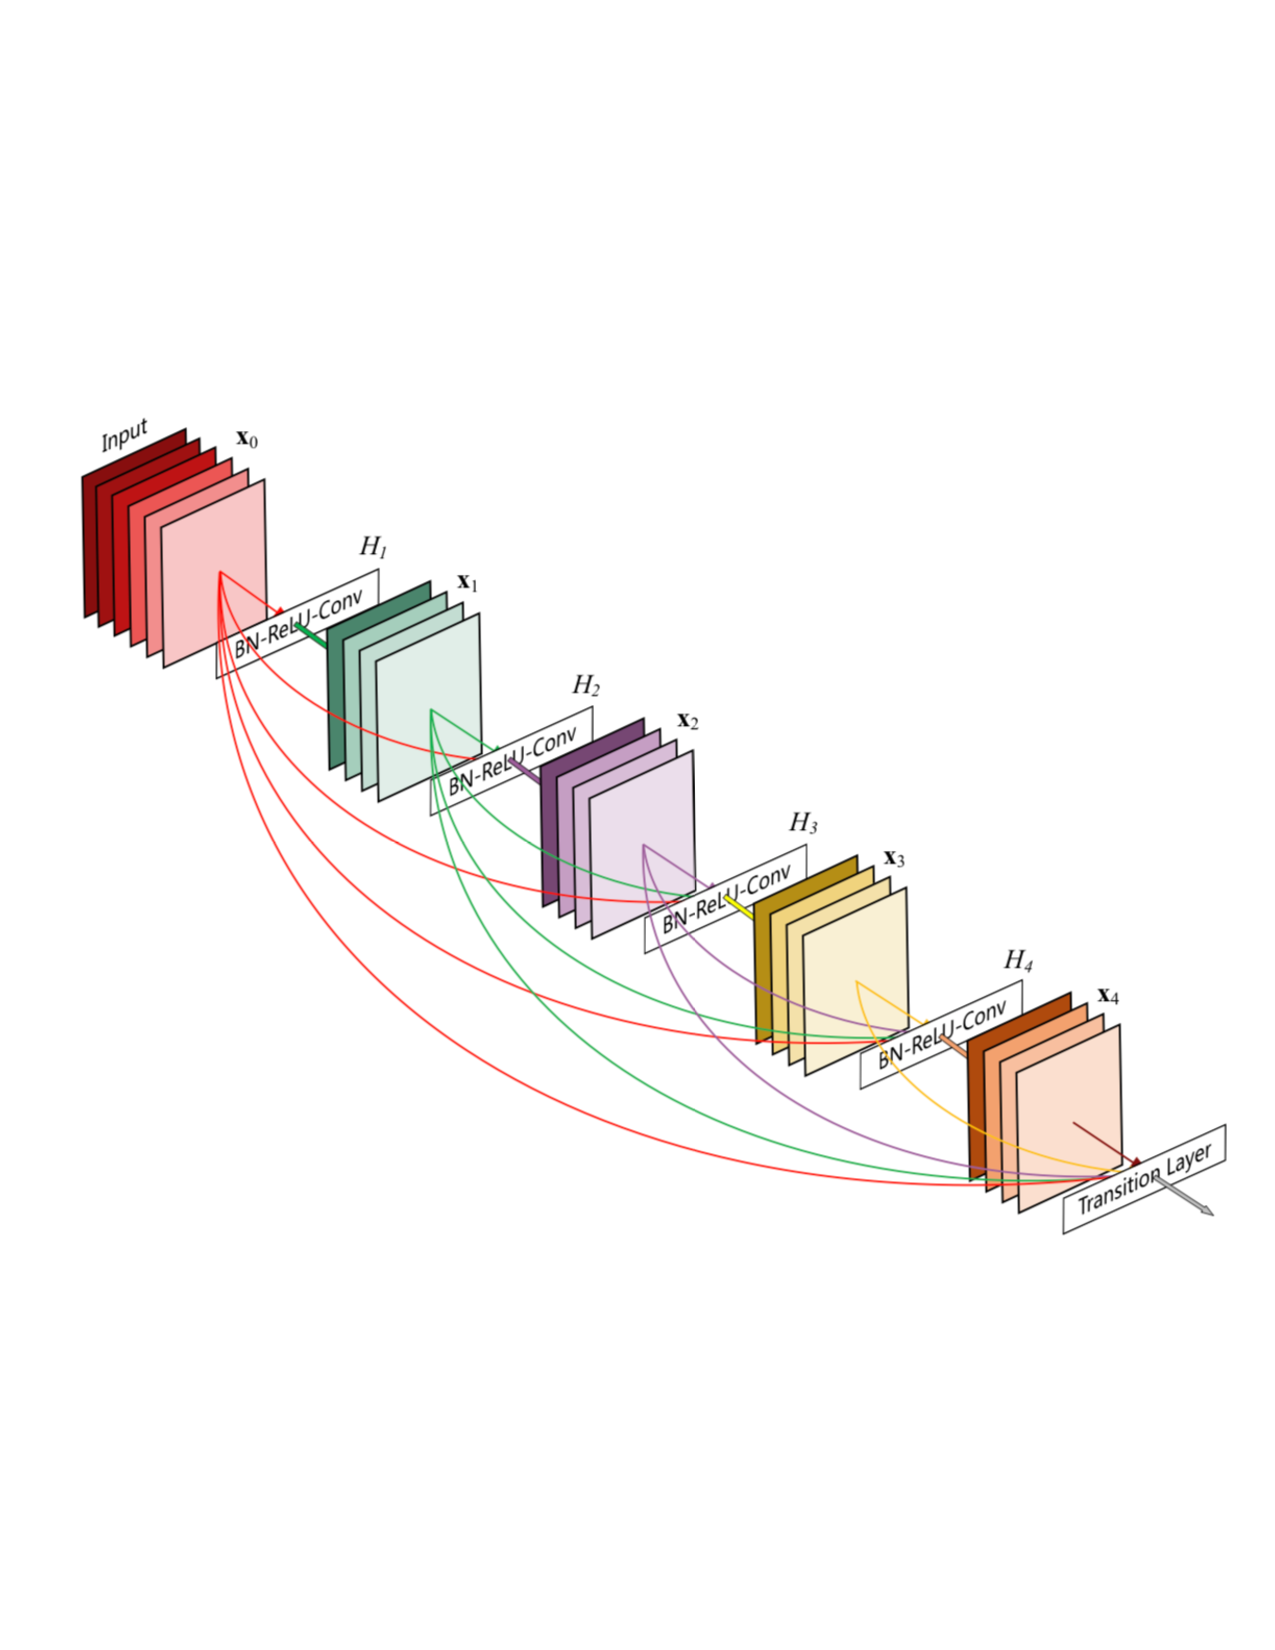
\includegraphics[width=\columnwidth]{figure_1}}
\caption{A 5-layer DenseBlock. Each layer takes all preceding feature-maps as input.}
\label{figure 1:}
\end{center}
\vskip -0.2in
\end{figure}

{\bf Multilabel setup.} I formulate the task as a multilabel classification problem. The disease labels for each image are represented as a 14-dimensional vector where each index corresponds to the presence of a disease. An image with no findings is represented as vector with all zeros. To enable multilabel classification, the final softmax layer in the DCNN is replaced by a sigmoid layer. This means that each disease is treated as a binary classification problem.

{\bf Localization.} To localize diseases in the images I used class activation mapping (CAM) \cite{Zhou}. This is a state of the art technique for unsupervised object localization. I did this by applying the logits layer to the DCNN output before global average pooling. I then resized this to 224 x 224 with bilinear interpolation. To generate bounding boxes for each class from the CAM, I then thresholded the heatmap at the value 0.9.

{\bf Increasing resolution.} To increase the resolution of the bounding box prediction I modified DenseNet-121. I did this by removing all the 2 x 2 average pooling layers. This increased the resolution of the DCNN output from 7 x 7 to 56 x 56 without increasing the number of parameters in the model.

{\bf Cross entropy loss.} Initially I used cross entropy loss, but the model struggled to learning positive instances, particularly for rare diseases. The remedy this, I switched to a weighted cross entropy loss like Wang et al \cite{Wang}. This uses a positive/negative balancing factor $ {\beta}_P $, $ {\beta}_N $
to ensure that equal weight it positive and negative examples in a given batch.
Weighted cross entropy loss (W-CEL) is defines as,
\begin{equation}
W-CEL = {\beta}_P\sum_{y_c=1}-ln(f(x_c)) + {\beta}_N\sum_{y_c=0}-ln(1-f(x_c))
\end{equation}
where $ {\beta}_P $ is set to $ \frac{|P| + |N|}{|P|} $ and $ {\beta}_N $ is set to $ \frac{|P| + |N|}{|N|} $.
$|P|$ and $|N|$ are the total number of 1s and 0s in the batch.

{\bf Localization loss.} For limited supervision with the bounding boxes I used cross entropy loss between the CAMs and bounding boxes. This was calculated only for the bounding boxes or for the bounding boxes and CAMs thresholded at the value 0.9.

\subsection{Training}

{\bf DCNN.} Both ResNet-50 and DenseNet-121 are implemented in TensorFlow using the TensorFlow-Slim framework. They are initialized with weights learned on the ImageNet dataset. Training is performed on a single Nvidia GPU, either a 1080 or P5000. The P5000 was needed to fit DenseNet-121 without average pooling.

{\bf Data augmentation.} Two data augmentation strategies were employed, horizontal flipping and horizontal flipping with random cropping. The random crops ranged in size from 100% to 50% of the image and were randomly distributed across the image.

{\bf Learning rate decay.} Two learning rate decay strategies were employed, gradual and step decay. Smooth decay decreased the learning rate by a factor of .94 every 2 epochs. Step decay decreased the learning rate by a factor of .1 every 10 epochs. The initial learning rate for both was .001.

{\bf Optimization.} Several optimization strategies were experimented with, but the most effective was Adam with the standard parameters (${\beta}1=.9$ and ${\beta}2=.999$). A batch size of 16 was used except for DenseNet-121 without average pooling. This architecture need a batch size of 8 to fit on a single GPU.

\section{Data}
\label{Data}

I used the chestXray-14 dataset which contains 112,120 frontal-view X-ray images of 30,805 unique patients \cite{Wang}.
Each image is labeled for 14 common thoracic diseases. The labels are extracted from radiology
reports and are estimated to be at least 90\% accurate. The dataset also includes 940 labeled
bounding boxes for 880 images which were generated by certified radiologists.
These are evenly split across 8 of the diseases in the dataset.
I resized the 3-channel image from 1024 x 1024 to 224 x 224 for faster processing
and normalized the pixel values for each channel to have the same mean and standard deviation as the images in ImageNet.

{\bf Unsupervised localization.} For the unsupervised localization experiments
I used the standard 70\% train, 10\% validation, and 20\% test split for the chestX-ray dataset.
There is no patient overlap between the splits. All the bounding boxes are in the test split.

{\bf Semi-supervised localization.} For the semi-supervised localization experiments
I split the chestX-ray dataset into 5 folds with 80\% train and 20\% test.
This was done with stratified random sampling so that there is the same number of
bounding boxes for each disease in each split. There is no patient overlap between the splits.

\section{Experiments and Results}
\label{Experiments and Results}

\subsection{Disease Identification}

{\bf ResNet.} I first established a baseline with ResNet to validate my code. This revealed a number of issues with my conversion of the dataset into TFRecord format. Once these were corrected I experimented with different loss functions and training techniques. I was able to achieve similar results to Wang et al., by just tuning the logits layer of a pretrained ResNet (figure 2) \cite{Wang}. Using weighted cross entropy loss like Wang et al., significantly increased the AUROC for less common diseases (figure 2). Fully tuning the pretrained ResNet slightly decreased the AUROC. This suggests that decent results can be achieved by using ResNet as a feature extractor and that is is difficult to fully train ResNet with the chestX-ray dataset.

\begin{figure}[p]
\vskip 0.2in
\begin{center}
\centerline{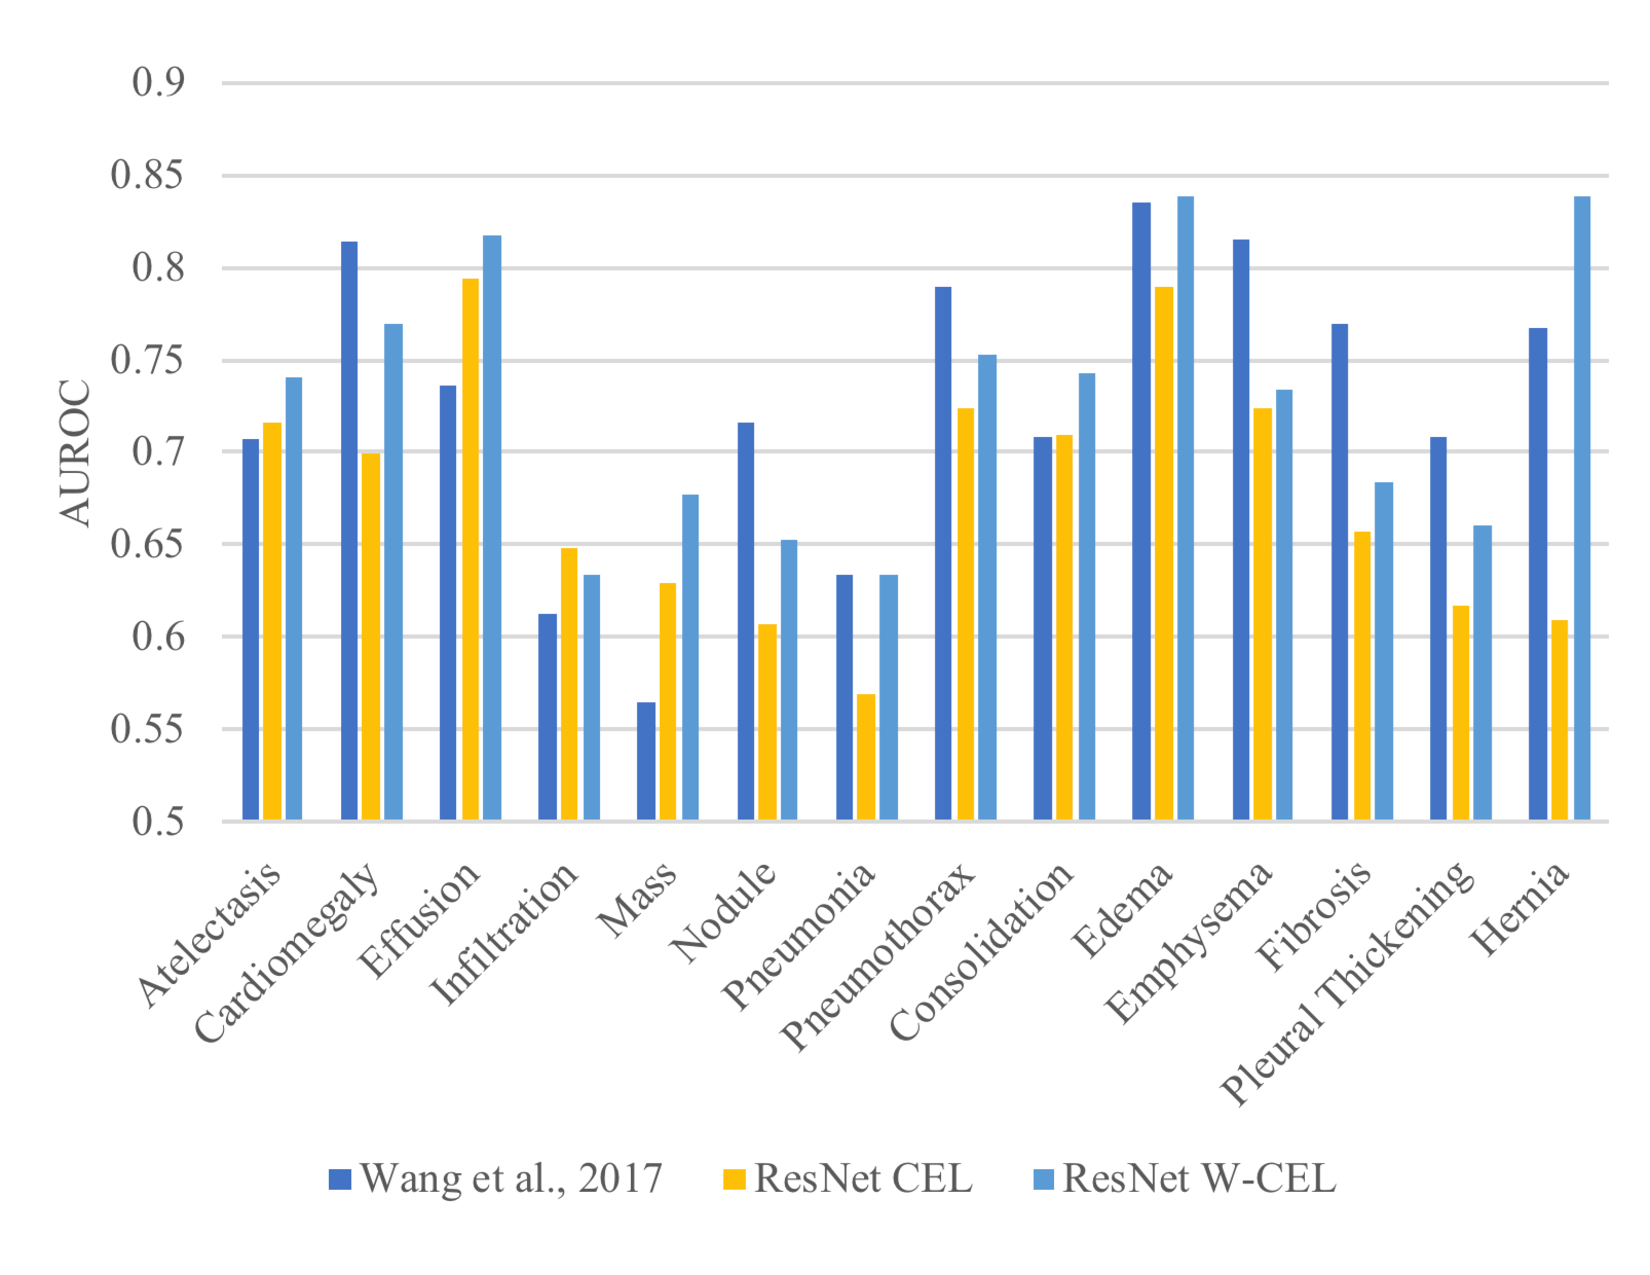
\includegraphics[width=\columnwidth]{figure_2}}
\caption{Comparison of ResNet to Wang et al., 2017. Using weighted cross entropy loss (W-CEL) increases the AUROC for less common diseases.}
\label{figure 2:}
\end{center}
\vskip -0.2in
\end{figure}

{\bf DenseNet.} To make training easier I used DenseNet. I experimented with a number of different optimizers, learning rate decay schedules, and data augmentation strategies. Experiments were run for 300,000 steps (75 epochs) to ensure convergence. For horizontal flipping and random cropping, adam was best with the gradual decay, and momentum was best with step decay. These had similar W-CEL and average AUROC values (figure 3). For horizontal flipping, step decay significantly outperformed gradual decay. This is likely because step decay prevents overfitting with less data augmentation. The W-CEL for the gradual decay is very low but this does not correspond to high average AUROC on the validation set (figure 3). Interesting, momentum converged faster than adam with step decay. My AUROC values are slightly worse than Rajpurkar et al \cite{Rajpurkar}. This is probably because I am doing multilabel classification instead of binary classification (figure 4).

\begin{figure}[p]
\vskip 0.2in
\begin{center}
\centerline{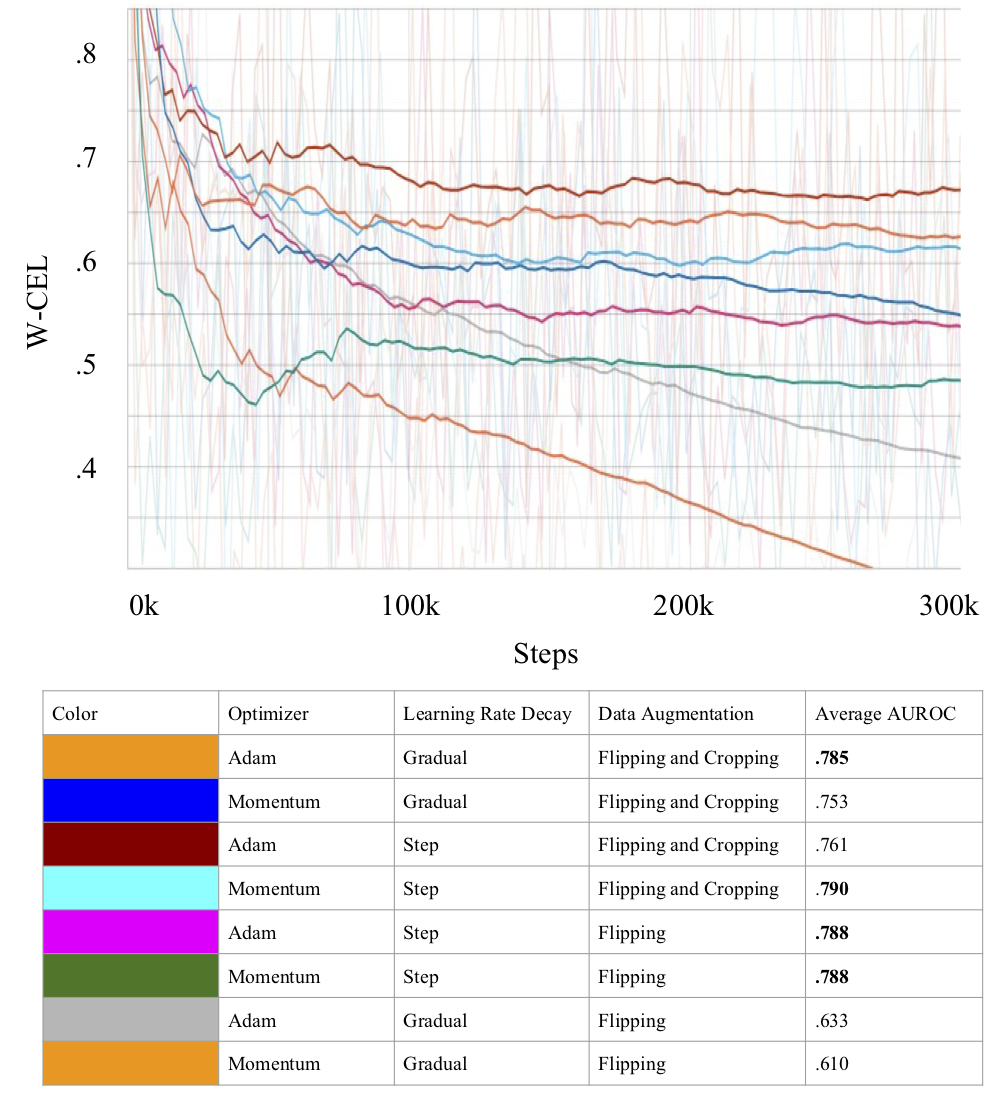
\includegraphics[width=\columnwidth]{figure_3A}}
\caption{Results for DenseNet with different optimizers, learning rate decay schedules, and data augmentation strategies.
The W-CEL is calculated with the training set and the AUROC is calculated with the test set.}
\label{figure 3:}
\end{center}
\vskip -0.2in
\end{figure}

\begin{figure}[p]
\vskip 0.2in
\begin{center}
\centerline{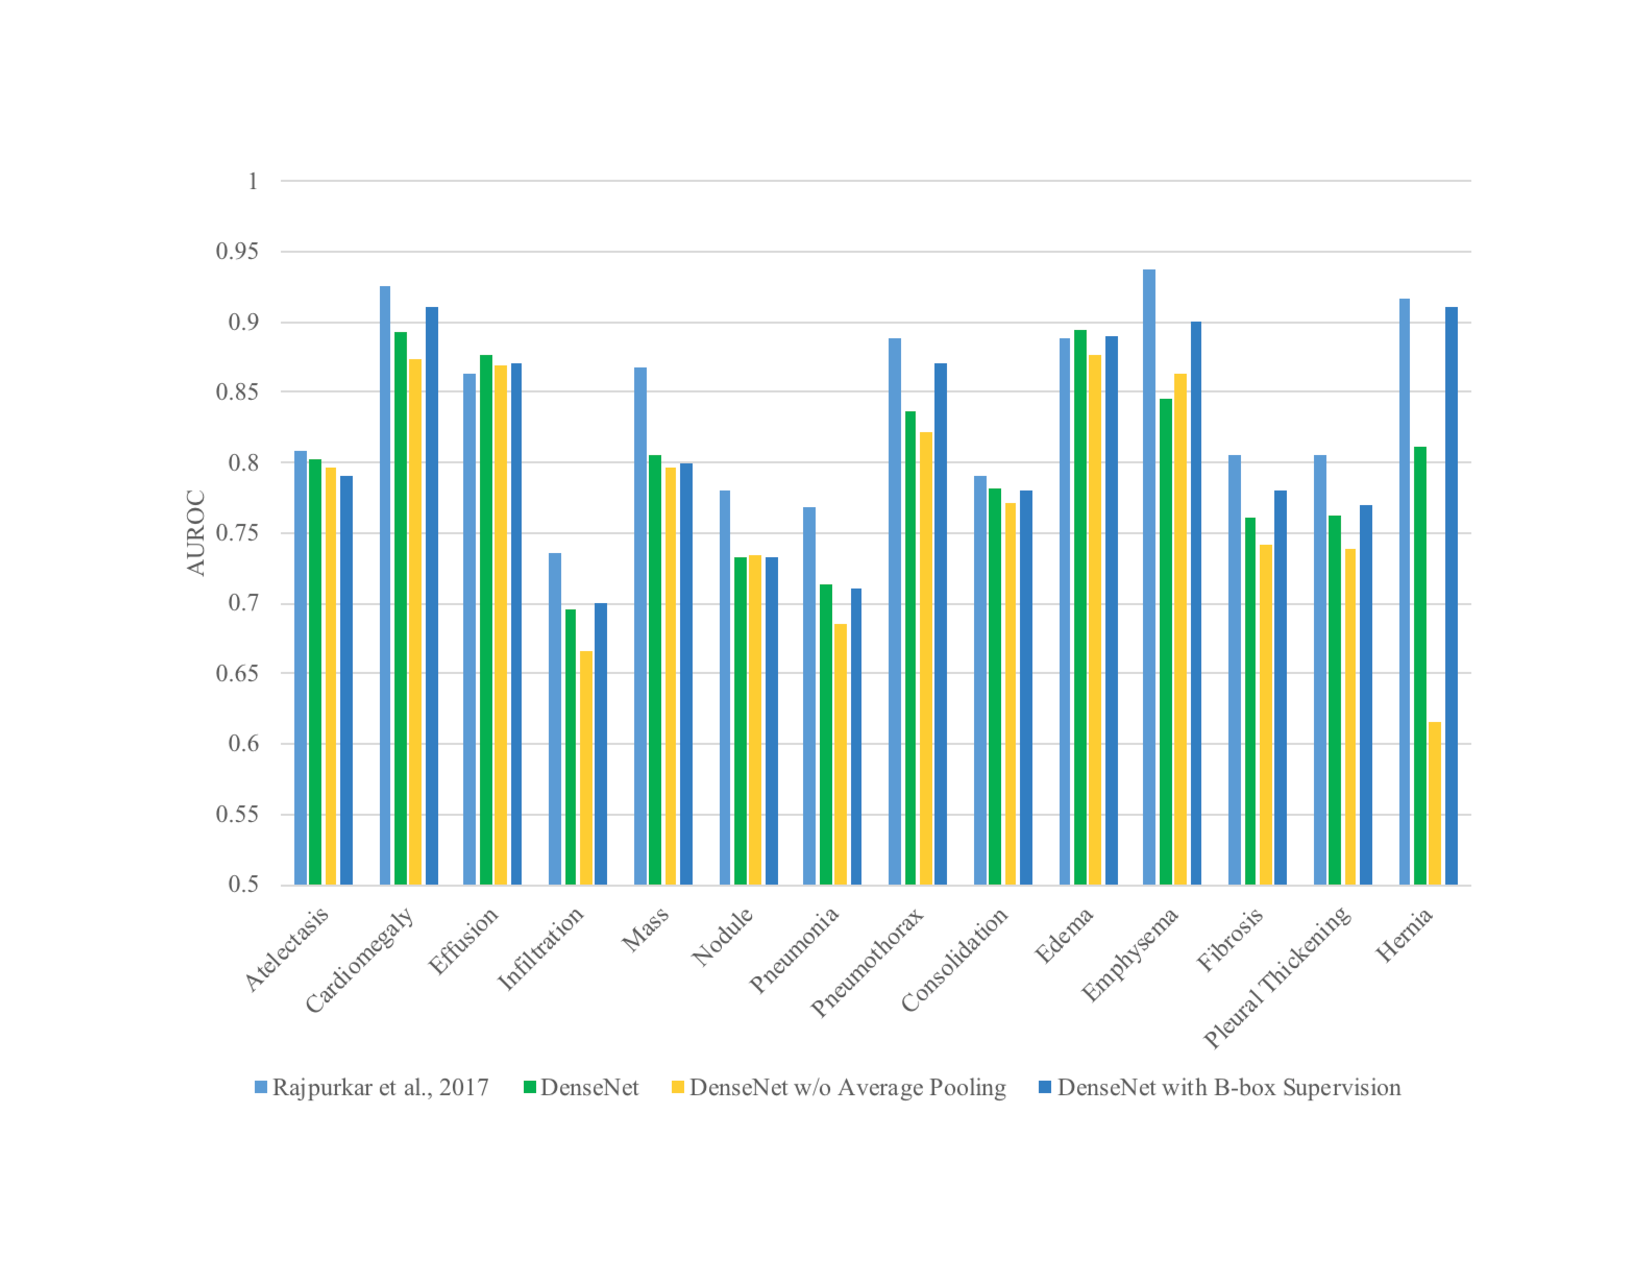
\includegraphics[width=\columnwidth]{figure_4}}
\caption{Comparison of DenseNet to Rajpurkar et al., 2017. Neither removing the average pooling layers nor supervising with bounding boxes effects the AUROC. The AUROC is calculated with the test set.}
\label{figure 4:}
\end{center}
\vskip -0.2in
\end{figure}

\subsection{Disease Localization}

{\bf CAMs.} To test the ability of DenseNet to localize diseases without bounding box supervision, I generated class activation maps (CAMs) \cite{Zhou}. These heatmaps were remarkably accurate for some images (figure 5). In these images, DenseNet focuses on small regions for localized diseases such as infiltration and nodule, and on larger regions for less localized diseases such as atelectasis and pleural thickening. I cannot truly validate these localizations since I am not a radiolist. For other images the heatmaps are diffuse and non-specific. In many of the images DenseNet focuses on medical devices and lines in the image. These are predictive of sick patients who are more likely to have a disease. This suggests that bounding box supervision is required for the localization of the disease instead of just regions which are predictive.

\begin{figure}[p]
\vskip 0.2in
\begin{center}
\centerline{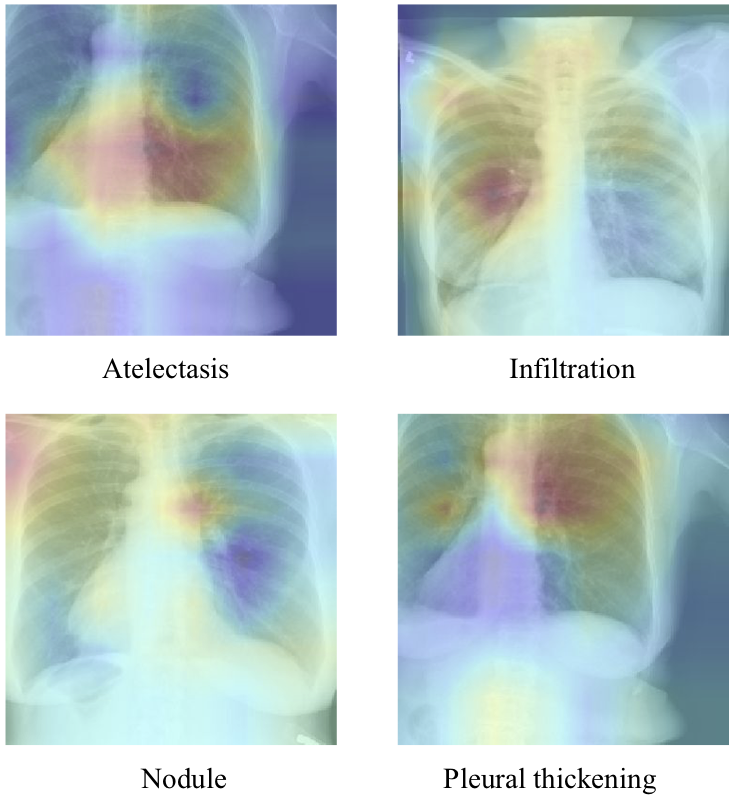
\includegraphics[width=\columnwidth]{figure_5}}
\caption{Example CAMs generated by DenseNet without bounding box supervision.}
\label{figure 5:}
\end{center}
\vskip -0.2in
\end{figure}

{\bf Bounding box locations.} Ideally, supervising with bounding boxes will improve identification as well as localization because it prevents overfitting to areas not associated with the disease and because the spatial location is indicative of the disease. To learn more about the spatial distribution of the bounding boxes I generated a heatmap for each disease with all the bounding boxes (figure 6). There are large differences in spatial deviation and size between diseases. For example, the bounding boxes for cardiomegaly are large and centered on the heart, while the bounding boxes for nodule are small and distributed throughout the lungs. It is clear that the localization is indicative for some diseases. For example, atelectasis is usually in the lower lungs and pneumothorax is usually in the upper lungs.

\begin{figure}[p]
\vskip 0.2in
\begin{center}
\centerline{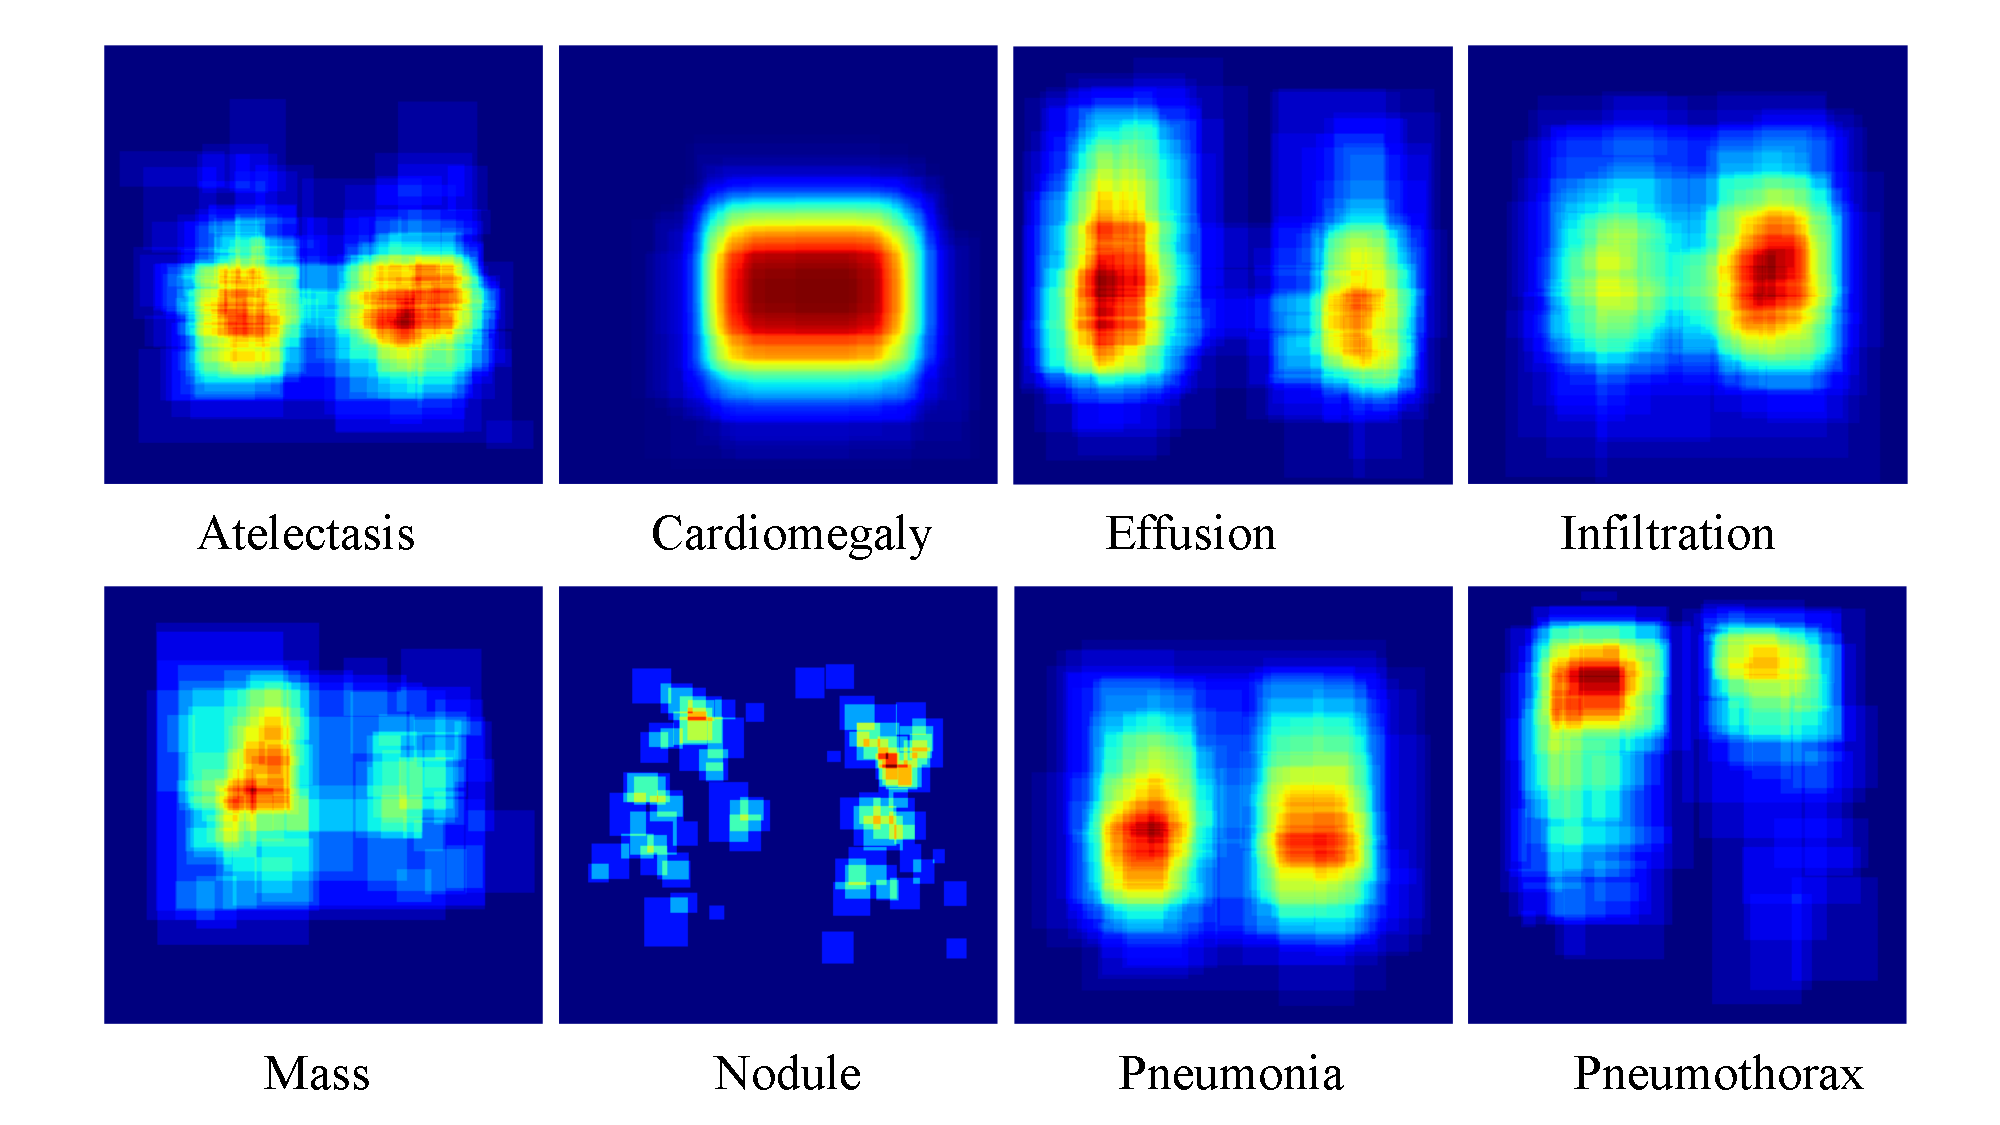
\includegraphics[width=\columnwidth]{figure_6}}
\caption{Spatial distribution of the bounding boxes across different diseases.}
\label{figure 6:}
\end{center}
\vskip -0.2in
\end{figure}

{\bf Semi-supervised localization.} To enable limited supervision by the bounding boxes I added localization loss to the total loss calculation. I experimented with calculating the localization loss only for the bounding boxes or for the bounding boxes and CAMs thresholded at the value 0.9. The point of including the thresholded CAMs was to stabilize the loss function, but this did not work. The model minimized the localization loss by predicting the disease was in the top left corner which did not negatively affect the identification loss. Just including the bounding boxes worked better. It significantly increased the IoU for most of the diseases and slightly improved the AUROC (figures 4,7). Some of the localization error appears to be caused by the low resolution (7 x 7) of the prediction. This is especially true for disease with small bounding boxes, like mass (figure 7).

\begin{figure}[p]
\vskip 0.2in
\begin{center}
\centerline{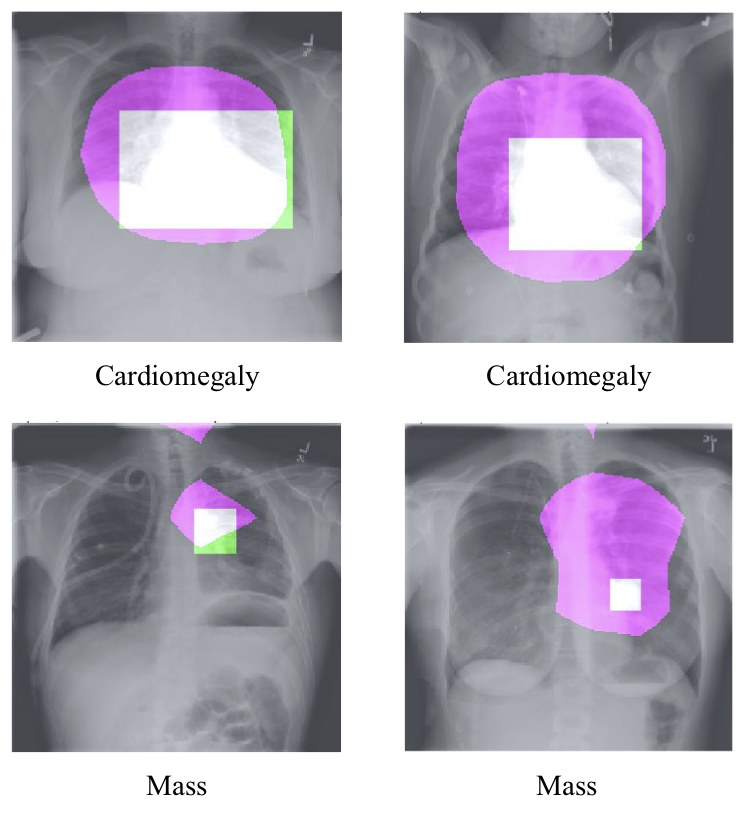
\includegraphics[width=\columnwidth]{figure_7}}
\caption{Localizations generated by bounding box supervised DenseNet compared to ground truth bounding boxes. Images are from the test set.}
\label{figure 7:}
\end{center}
\vskip -0.2in
\end{figure}

\begin{figure}[ht]
\vskip 0.2in
\begin{center}
\centerline{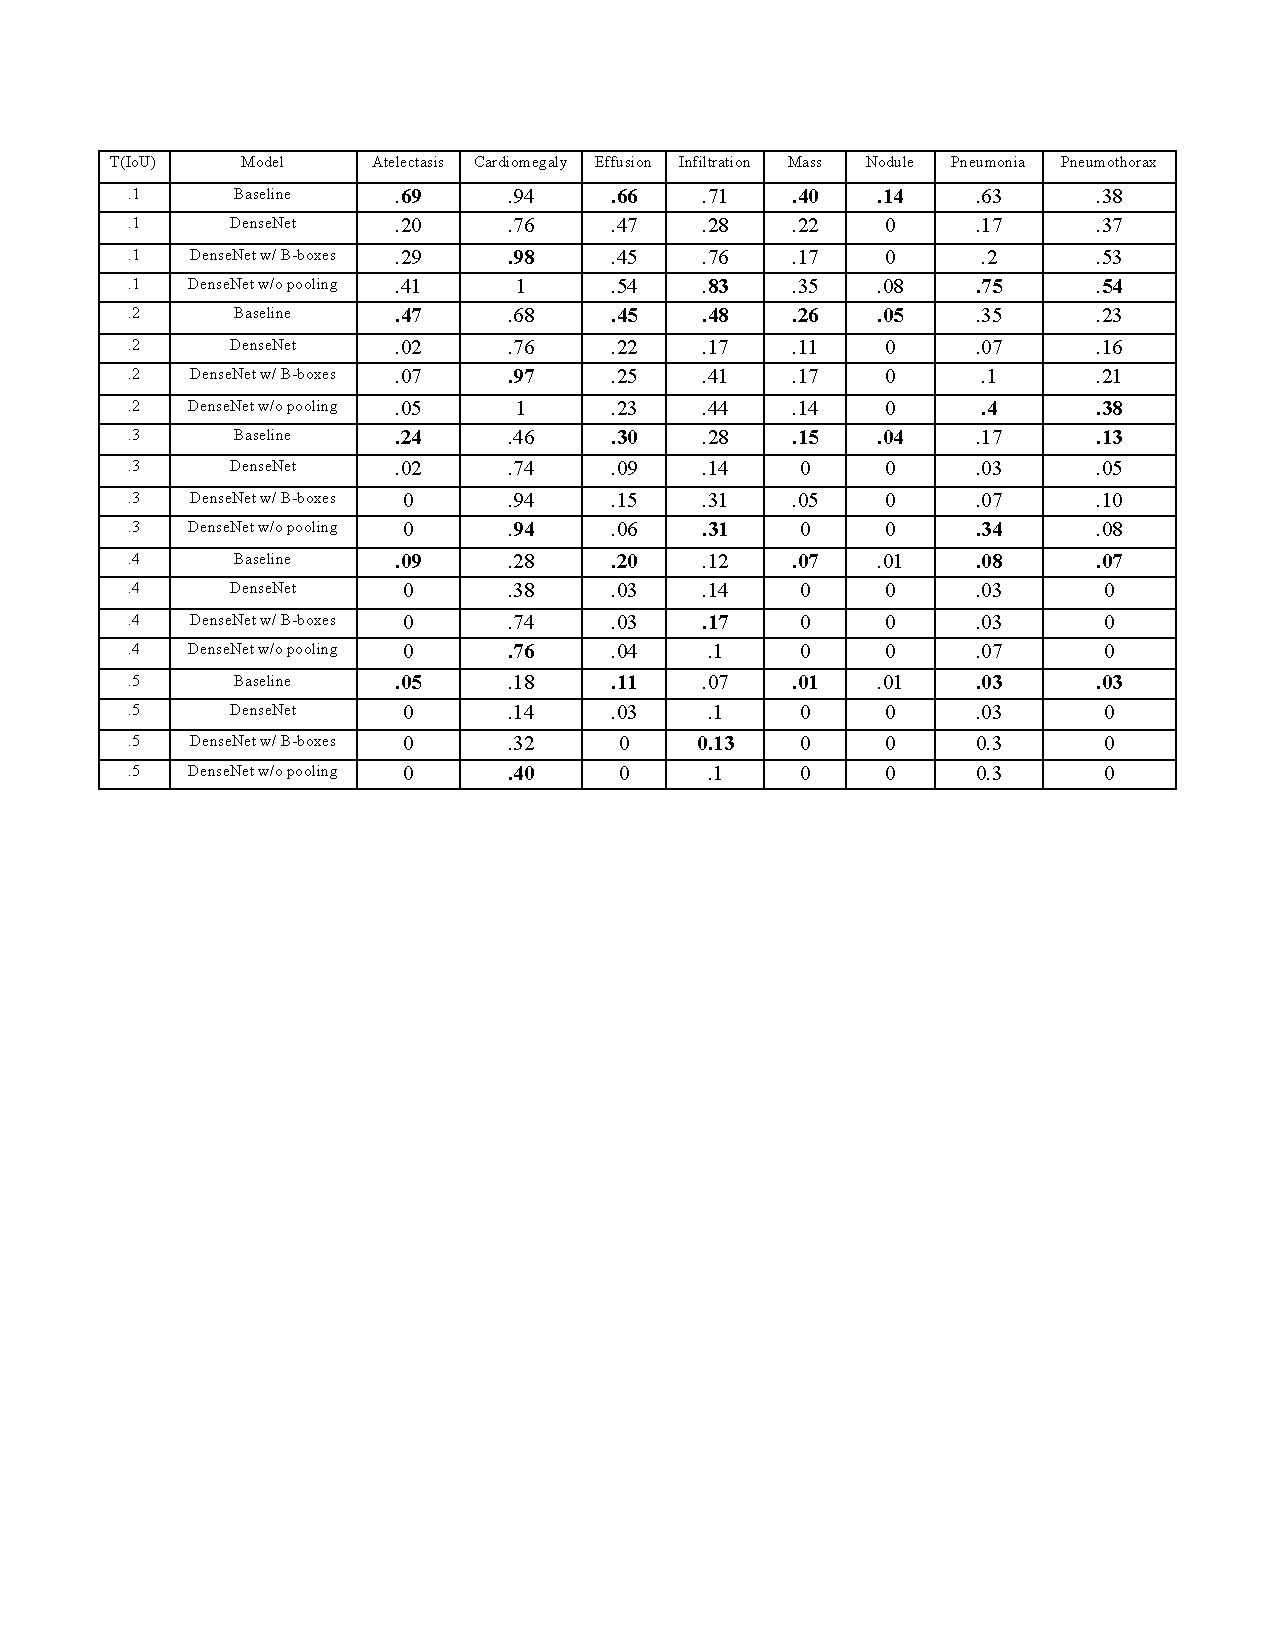
\includegraphics[width=\columnwidth]{figure_8}}
\caption{Accuracy at IoU = [.1,.2,.3,.4,.5] for Wang et al., 2017, DenseNet, DenseNet with bounding box supervision, and DenseNet without average pooling}
\label{figure 8:}
\end{center}
\vskip -0.2in
\end{figure}

{\bf Increasing resolution.} To increase the resolution of the prediction I removed the 2 x 2 average pooling layers from DenseNet. This increased the time needed to train the model by a factor of 4. I trained this model with limited supervision from the bounding boxes like the lower resolution model. This yielded a slightly lower AUROC but significantly increased the IoU (figures, 4,8). The IoU values are comparable to the baseline established by Wang et al. However, Li et al. achieved significantly better localization. This is likely because I have not tuned the weight of the localization loss. Li et al scaled the localization loss by 5 since there are only a few bounding boxes \cite{Li}. I also have not done 5-fold cross validation, which is probably why the IoU for nodule is really low. There are only a few examples of nodules in the test set and I am getting them all wrong.

\section{Conclusions}

In conclusion, I achieve near state of the art identification of thoracic diseases by training a 121-layer DenseNet on the chestX-ray dataset \cite{Rajpurkar}. This task is formulated as a multilabel classification problem and I use a weighted loss function to insure the that the model learns to identify rare diseases. I achieve similar localization results to Wang et al without an post processing \cite{Wang}. I do this by training the model with limited supervision from the bounding boxes and removing the 2 x 2 average pooling layers to increase the resolution. My IoU values are generally low and do not compare to the state of the art.

\section{Future Directions}

This project is far from complete. My results so far provide a framework for the development of more complex models. Much of what I have done is similar to previous papers. In the future, I will focus on the increasing the ability of the model to localize diseases, since this is essential for computer aided diagnosis. I will do this by tuning the weight of the localization loss and possibly using a conditioned random field to iteratively generate ground truth bounding boxes for images without bounding boxes during training. Results similar to supervised localization have been reported using this technique \cite{Li2}. I will also work on increasing the resolution of the heatmap without significantly increasing the training time. This could be accomplished using a U-Net which takes the low resolution heatmap and the scales it back up using deconvolution layers and skip connecting to higher resolution feature maps \cite{Ronneberger}. The ultimate goal is to have a network which can accurately localize small abnormalities, like nodules.

\section*{Acknowledgments}

I would like to thank Ameet Soni for mentorship and guidance throughout this project me and Jeff Knerr his technical support.


\bibliography{references}
\bibliographystyle{icml2014}

\end{document}


% This document was modified from the file originally made available by
% Pat Langley and Andrea Danyluk for ICML-2K. This version was
% created by Lise Getoor and Tobias Scheffer, it was slightly modified
% from the 2010 version by Thorsten Joachims & Johannes Fuernkranz,
% slightly modified from the 2009 version by Kiri Wagstaff and
% Sam Roweis's 2008 version, which is slightly modified from
% Prasad Tadepalli's 2007 version which is a lightly
% changed version of the previous year's version by Andrew Moore,
% which was in turn edited from those of Kristian Kersting and
% Codrina Lauth. Alex Smola contributed to the algorithmic style files.
